\documentclass{beamer}
\setbeamerfont{caption}{size=\tiny}

\usepackage{graphicx}
\usepackage{xcolor}
\usepackage{subcaption}
\usepackage{tabularx}
\usepackage{hyperref}
\usepackage{amssymb,amsmath,amsthm}

\graphicspath{{../images/}}

\defbeamertemplate*{title page}{customized}[1][]
{
  \begin{center}
    \usebeamerfont{institute}\Huge\insertinstitute\par      
  \end{center}
  \centering
  \usebeamerfont{title}\LARGE\inserttitle\par
  \usebeamerfont{subtitle}\Large\insertsubtitle\par
  \bigskip
  \small\usebeamerfont{author}\insertauthor\par
  \usebeamerfont{date}\insertdate\par
}


\institute{Alma Mater Studiorum \\ University of Bologna}
\title{Artificial Intelligence - Machine Learning for Computer Vision}
\subtitle{Project work}
\author{Alessandro Dicosola [Matr. 935563]}
\date{}


\begin{document}
\begin{frame}
    \titlepage
\end{frame}

\begin{frame}{Task}
    SR is an \textcolor{red}{Ill-posed problem}: trying to create a mapping between LR to HR for \textcolor{blue}{reconstructing} SR images
    
    Keywords: super-sampling, super-resolution.
\end{frame}

\begin{frame}{Related works}{SR through internal and external database\cite[Releated works]{LapSRN}}
    \small
    Exploit similarity between textures in images therefore create pairs of LR-HR patches for learning a low dimensional space were apply k-NN, non linear regressor, random forest, ... ,

    manifold embedding\cite[2004]{SRneighbporembedding}:
    \begin{columns}
        \begin{column}{0.5\textwidth}
            \begin{itemize}
                \tiny
                \item LR patches embedding is the concatenation of the first and second order derivative of the luminance at each pixel on the patch in the YIQ domain. 
                \item HR patches embedding is the concatenation of all luminance at each pixel
                \item Given a LR patch find the k-NN patches on the training set $$N_q$$
                \item Compute the reconstruction weights minimizing the reconstruction error: $$argmin_W || x_t^q - \sum_{x_s^p \in N_q} w_{qp}x_s^p ||^2$$
                \item Reconstruct the HR patch: $$y_t^q = \sum_{x_s^p \in N_q} w_{qp}y_s^p$$
                \item Reconstruct the image overlapping the patches ( averaging on overlapped regions)
            \end{itemize}            
        \end{column}
        \begin{column}{0.5\textwidth}
            
            \begin{figure}
                \centering
                \begin{subfigure}[l]{0.55\textwidth}
                    \vspace*{-50px}
                    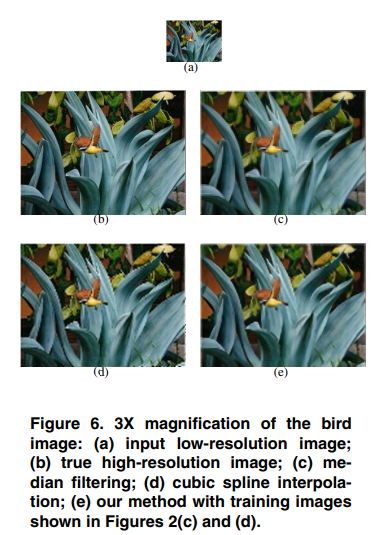
\includegraphics[height=0.30\textheight, keepaspectratio]{result-neighbour-embedding.png}
                \end{subfigure}
                \begin{subfigure}[l]{0.55\textwidth}
                    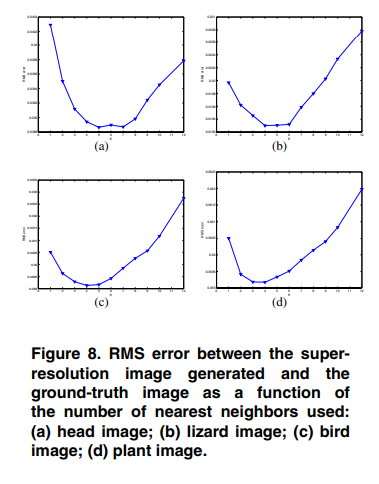
\includegraphics[height=0.30\textheight, keepaspectratio]{rms-neighbour-embedding.png}                    
                \end{subfigure}
            \end{figure}
        \end{column}
    \end{columns}
\end{frame}

\begin{frame}{Releated works}{CNN \cite[Releated works]{ASDN} \cite{SRsurvey}}
    \begin{itemize}
        \item SRCNN \cite{srcnn} : CNN using only three convolutions for extracting information, process them and reconstruct the SR image.
        \item VDSR : VGG-net that learns a residual instead of the direct mapping LR-HR in order to focus the training on high frequency information.
        \item SRDenseNet, RDN, \textcolor{red}{DBDN\cite{DBDN}}: Combine residual connection (locally and globally) with dense connection
        \item \textcolor{red}{RCAN\cite{RCAN}}, \textcolor{red}{CSFM\cite{spatialattentionmechanism9}} : Use channel-wise and spatial attention for focusing the training on important features or region in order to ease the convergence and improve the results.
        \item \textcolor{red}{LapSRN\cite{LapSRN}}, \textcolor{red}{MS-LapSRN\cite{MSLapSRN}} : multi scale network using a \textit{Laplacian Pyramid Framework} \cite{laplacianpyramid}
        \item \textcolor{red}{MetaSR\cite{MetaSR}} : use a meta-upscaling module for learning LR-HR mapping using any scale.
    \end{itemize}
\end{frame}

\begin{frame}{ASDN - Arbitrary-Scale Deep Network}
    \only<1>{
        \begin{itemize}
            \item Find an LR-HR mapping with \textcolor{blue}{any} scale (integer or real)
            \item Use Laplacian Frequency Representation \cite{laplacianpyramid} for reconstructing SR image interpolating two nearest level in the LFR.
            \item The range scales was found to be optimal between 1 and 2 using 11 levels in the LFR.
            \item For scale greater than 2 the network is \textit{deployed recursively}.
        \end{itemize}
    }

    \only<2>{
        \framesubtitle{Laplacian Frequency Representation}
        \begin{figure}
            \centering
            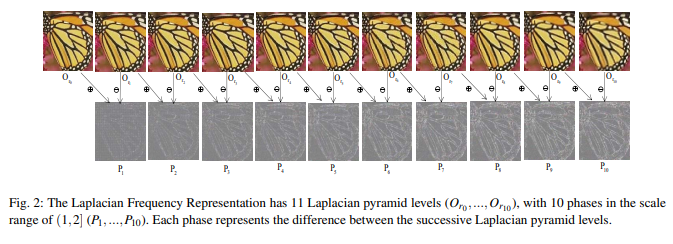
\includegraphics[height=0.3\textheight, keepaspectratio]{asdn-laplacian-pyramid.png}
        \end{figure}
        \begin{itemize}
            \item Learning any decimal scale is not possible: infinite decimal scales.
            \item Reconstruct the SR image interpolating the two nearest level in the LFR.
            \item Each level learn the HR representation at particular scale in the range.
            \item Compute the \textit{phase} as the difference between two consecutive levels in order to acquire \textbf{high frequency information}: $$ P_i = O_{r_{i-1}} - O_{r_i} $$
        \end{itemize}
    }

    \only<3>{
        \framesubtitle{Laplacian Frequency Representation}
        \begin{itemize}
            \item The scale for each level is:
            $$r_l = \frac{l}{L-1} + 1$$
            therefore the level can be indexed as
            $$l = (r_l - 1) * (L-1)$$
            $$i = \left\lceil (r - 1) * (L - 1) \right\rceil $$
            \item Define the weight, proportional to the distance between the scales, as:
            $$w_r = (L - 1)*(r_i - r)$$
            \item The SR image is reconstructed as:
            $$O_r = O_{r_i} + w_r \ast P_i $$
        \end{itemize}
    }
    \only<4>{
        \framesubtitle{Example}
        $$r = 1.27$$
        $$i = \left\lceil 10 * (1.27 - 1)\right\rceil = \left\lceil2.7\right\rceil = 3$$
        $$w_r = 10 * (1.3 - 1.27) = 0.3$$
        $$O_r = O_{r_3} + 0.3 \ast P_3$$
    }
    \only<5>{
        \framesubtitle{Recursive deployment}
        \begin{itemize}
            \small
            \item Learning the mapping for any scale is too complex.
            \item For scales greater than the maximum in the scale range apply recursively the network.
            \item A large scale \textit{R} can be expressed as an integer \textit{N} power of decimal ratio \textit{r}:
            $$R = r^N \Rightarrow N= \log_r R$$
            \item Was found that using the greatest r at the beginning lead to better performance
            \item Since the range is fixed between (1,2] then $$\left\lceil N=\log_2 R \right\rceil$$ and therefore
            $$r_i = 
            \begin{cases}
                2 & \text{i } \le \text{N - 1} \\
                \frac{R}{2^{N-1}} & \text{i}=\text{N} \\
            \end{cases}
            $$
        \end{itemize}
    }  
\end{frame}

% EXTRA 
\begin{frame}{Extra}{Laplacian pyramid\cite{laplacianpyramid}}
    \begin{itemize}
        \small
        \item Generate images with high frequency information only subtracting two consecutive levels in the Gaussian-like pyramid. 
        \item Those images can be used for reconstructing the original image.
        \item Hand crafted kernel for filtering the image in order to cutoff low frequency (low-pass filtering) information:
        \begin{itemize}
            \tiny
            \item Separable
            \item Symmetric
            \item Normalized: $$a + 2b + 2c = 1$$
            \item Equal contribution: $$a + 2c = 2b$$
            \item Kernel = 
        \end{itemize}
    \end{itemize}
    \begin{columns}
        \begin{column}{0.3\textwidth}
            \begin{figure}
                \centering
                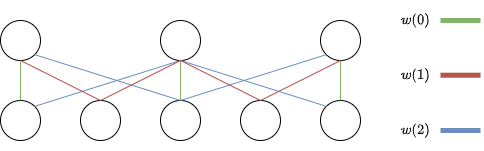
\includegraphics[scale=0.2]{laplacianpyramidexample.png}
                \caption{Equal contribution.}
            \end{figure}        
        \end{column}
        \begin{column}{0.6\textwidth}
            \begin{itemize}
                \tiny
                \item All nodes in the lower level must have the same contribution to nodes in the upper level. 
                \item The central node contributes with a + 2c
                \item The middle ones contribute with 2b
                \item The outer ones with a + c
                \item So a+2c=2b
            \end{itemize}
        \end{column}
    \end{columns}    
\end{frame}

\bibliographystyle{ieeetr}
\bibliography{../bibliography}

\end{document}